%%%%%%%%%%%%%%%%%%%%%%%%%%%%%%%%%%%%%%%%%%%%%%%%%%%%%%%%%%%%%%%%%%%%%%%%%%%%%%%%
%%%%%%%%%%%%%%%%%%%%%%%%%%%%%%%%%%%%%%%%%%%%%%%%%%%%%%%%%%%%%%%%%%%%%%%%%%%%%%%%
%%% Template for AIMS Rwanda Assignments         %%%              %%%
%%% Author:   AIMS Rwanda tutors                             %%%   ###        %%%
%%% Email: tutors2017-18@aims.ac.rw                               %%%   ###        %%%
%%% Copyright: This template was designed to be used for    %%% #######      %%%
%%% the assignments at AIMS Rwanda during the academic year %%%   ###        %%%
%%% 2017-2018.                                              %%%   #########  %%%
%%% You are free to alter any part of this document for     %%%   ###   ###  %%%
%%% yourself and for distribution.                          %%%   ###   ###  %%%
%%%                                                         %%%              %%%
%%%%%%%%%%%%%%%%%%%%%%%%%%%%%%%%%%%%%%%%%%%%%%%%%%%%%%%%%%%%%%%%%%%%%%%%%%%%%%%%
%%%%%%%%%%%%%%%%%%%%%%%%%%%%%%%%%%%%%%%%%%%%%%%%%%%%%%%%%%%%%%%%%%%%%%%%%%%%%%%%


%%%%%% Ensure that you do not write the questions before each of the solutions because it is not necessary. %%%%%% 

\documentclass[12pt,a4paper]{article}

%%%%%%%%%%%%%%%%%%%%%%%%% packages %%%%%%%%%%%%%%%%%%%%%%%%
\usepackage{amsmath}
\usepackage{amssymb}
\usepackage{amsthm}
\usepackage{amsfonts}
\usepackage{graphicx}
\usepackage[all]{xy}
\usepackage{tikz}
\usepackage{verbatim}
\usepackage[left=2cm,right=2cm,top=3cm,bottom=2.5cm]{geometry}
\usepackage{hyperref}
\usepackage{caption}
\usepackage{subcaption}
\usepackage{psfrag}

%%%%%%%%%%%%%%%%%%%%% students data %%%%%%%%%%%%%%%%%%%%%%%%
\newcommand{\student}{Akor Stanley}
\newcommand{\course}{PDE1 }
\newcommand{\assignment}{1}

%%%%%%%%%%%%%%%%%%% using theorem style %%%%%%%%%%%%%%%%%%%%
\newtheorem{thm}{Theorem}
\newtheorem{lem}[thm]{Lemma}
\newtheorem{defn}[thm]{Definition}
\newtheorem{exa}[thm]{Example}
\newtheorem{rem}[thm]{Remark}
\newtheorem{coro}[thm]{Corollary}
\newtheorem{quest}{Question}[section]

%%%%%%%%%%%%%%  Shortcut for usual set of numbers  %%%%%%%%%%%

\newcommand{\N}{\mathbb{N}}
\newcommand{\Z}{\mathbb{Z}}
\newcommand{\Q}{\mathbb{Q}}
\newcommand{\R}{\mathbb{R}}
\newcommand{\C}{\mathbb{C}}
%%%%%%%%%%%%%%%%%%%%%%%%%%%%%%%%%%%%%%%%%%%%%%%%%%%%%%%555
\begin{document}
%%%%%%%%%%%%%%%%%%%%%%% title page %%%%%%%%%%%%%%%%%%%%%%%%%%
\thispagestyle{empty}
\begin{center}
\textbf{AFRICAN INSTITUTE FOR MATHEMATICAL SCIENCES \\[0.5cm]
(AIMS RWANDA, KIGALI)}
\vspace{1.0cm}
\end{center}
%%%%%%%%%%%%%%%%%%%%% assignment information %%%%%%%%%%%%%%%%
\noindent
\rule{17cm}{0.2cm}\\[0.3cm]
Name: \student \hfill Assignment Number: \assignment\\[0.1cm]
Course: \course \hfill Date: \today\\
\rule{17cm}{0.05cm}
\vspace{1.0cm}
\section*{Question 1}
\begin{itemize}
\item[(a)]
For $y_{1}(x)$ and $y_{2}(x)$ to be independent, their wronskian given by; $W[y_{1}(x),y_{2}(x)](x) \neq 0$ for some values of $x$.\\
\newline
Given;
\begin{align}
\tilde{y_{1}}(x)&=ay_{1}+ay_{2}\\ \label{2}
\tilde{y_{2}}(x)&=cy_{2}+dy_{2} \\\label{3}
 \end{align}	
$W[\tilde{y_{1}}(x), \tilde{y_{2}}(x)]$=$\tilde{y_{1}}(x)\tilde{y_{2}}^{\prime}(x)$ -$\tilde{y_{2}}(x)\tilde{y_{1}}^{\prime}(x)$,\\
\newline
Where:	
\begin{align}
\tilde{y_{1}}^{\prime}(x)&=ay_{1}^{\prime}+by_{2}^{\prime}\\
\tilde{y_{2}}^{\prime}(x)&=cy_{2}^{\prime}+dy_{2}^{\prime}
\end{align}
Therefore:\\
\begin{align}
W[\tilde{y_{1}(x)},\tilde{y_{2}}(x)](x)&=(ay_{1}+ay_{2})(cy_{2}^{\prime}+dy_{2}^{\prime})-(cy_{2}+dy_{2})(ay_{1}^{\prime}+by_{2}^{\prime})\\
&=(ad-bc)(y_{1}y_{2}^{\prime}-y_{2}y_{1}^{\prime})\\
&=(ad-bc)W[y_{1}(x),y_{2}(x)]\label{1}
\end{align}
From our Previous statement, we have established that for $y_{1}$ and $y_{2}$ to be independent, $W[y_{1}(x),y_{2}(x)](x) \neq 0$. From equation(\ref{1}) we can deduce that;\\
\newline
$W[\tilde{y_{1}(x)},\tilde{y_{2}}(x)]$, $\therefore$ (ad-bc) $\neq$ 0

\item[(b)]The Green's function $G(x,s)$ is given by;
\begin{align*}
G(x,s)=\frac{\tilde{y_{1}}(s)\tilde{y_{2}}(x)-\tilde{y_{2}}(s)\tilde{y_{1}}(x)}{W[\tilde{y_{1}},\tilde{y_{2}}](s)},
\end{align*}
Substituting the values of $\tilde{y_{1}}$ and $\tilde{y_{2}}$ given in equations(\ref{2},\ref{3}) and the expression for the Wronskian given in equation(\ref{1}). We shall obtain;\\ 
\begin{align*}
G(x,s)&=\frac{(ad-bc)(y_{1}(S)y_{2}(x)-y_{2}(S)y_{1}(x))}{(ad-bc)W[y_{1},y_{2}](s)}\\
&=\frac{y_{1}(S)y_{2}(x)-y_{2}(S)y_{1}(x)}{W[y_{1},y_{2}](s)}\\
&=G(x,s)
\end{align*}
In conclusion, the Green function obtained from $\tilde{y_{2}}(x)$ and $\tilde{y_{1}}(x)$, is the same as that of $y_{1}$ and $y_{2}$.

\item[(c)]
\begin{align*}
{y^{\prime}}^{\prime}-4y^{\prime}+4y=r(x) \quad \quad\quad\quad\quad\quad y(0)=0, \quad y^{\prime}=0
\end{align*}
To solve the equation above, we first consider the homogeneous case given below;\\
\begin{align*}
{y^{\prime}}^{\prime}-4y^{\prime}+4y=0
\end{align*}
By assuming that $y=e^{mx}$ is a solution, we obtain the following characteristics equation.
\begin{align}
m^{2}-4m+4&=0 \label{4}
\end{align}
Solving the quadratic equation given in equation(\ref{4}) yields $m_{1}=2$ and $m_{2}=2$, the solution of the homogeneous part is given by;\\
$$ y_{1}=e^{2x} \quad \quad  y_{2}=xe^{2x} $$
The Wronskian is given by $W[y_{1}(x),y_{2}(x)]=y_{2}^{\prime}y_{1}-y_{1}^{\prime}y_{1}$\\
Where;\\
\begin{align*}
y_{1}^{\prime}&=2e^{2x}\\
y_{2}^{\prime}&=e^{2x}+2xe^{2x}
\end{align*}
$\therefore$ $W[y_{1}(x),y_{2}(x)]=(e^{2x}+2xe^{2x})e^{2x}-2e^{2x}(xe^{2x})=e^{4x}$.\\
\newline
The Green function $G(x,s)$ is given by;
\begin{align*}
G(x,s)&=\frac{y_{1}(s)y_{2}(x)-y_{2}(s)y_{1}(x)}{W[y_{1},y_{2}](s)}\\
&=\frac{e^{2s}xe^{2x}-se^{2s}e^{2x}}{e^{4s}}\\
&=xe^{2x}e^{-2s}-se^{-2s}e^{2x}\\
&=(x-s)e^{2x-2s}
\end{align*}
The particular solution $y_{p}$ of the differential equation can be obtained by  using the following approach.
\begin{align*}
y_{p}&=\int ^{s}\limits_{x=0}r(s)G(x,s)ds\\
&=\int ^{s}\limits_{x=0} se^{2s}(x-s)e^{2x-2s}ds\\
&=xe^{2x}\int ^{s}\limits_{x=0}sds- e^{2x}\int ^{s}\limits_{x=0} s^{2}ds\\
&=xe^{2x}(\frac{x^{2}}{2})-e^{2x}(\frac{x^{3}}{3})\\
&=\frac{x^{3}e^{2x}}{6}
\end{align*}
\end{itemize}
\section*{Question 2}
\begin{align}
\frac{d^{2}y}{dx^{2}}&=\lambda y \label{5}\\ 
y^{\prime}(1)&=0\\ 
y(0)&=0
\end{align}
\begin{itemize}
	\item [(a)] 
	\begin{align}
	\int^{1}\limits_{0}(y_{m}(x){y^{\prime}}^{\prime}_{n}-y_{n}(x){y^{\prime}}^{\prime}_{m}dx=0 \label{6}
	\end{align}
By applying integration by parts, $\int uv^{\prime}=uv-\int v du$.\\
Where;\\
$u_{1}=y_{m}(x)$, $v^{\prime}_{1}={y^{\prime}}^{\prime}_{n}$, $v_{1}=y^{\prime}_{n}$ and $du_{1}=y^{\prime}_{m}dx$  \\
$u_{2}=y_{n}(x)$ and $v^{\prime}_{2}={y^{\prime}}^{\prime}_{m}$, $v_{1}=y^{\prime}_{m}$ and $du_{1}=y^{\prime}_{n}dx$
\begin{align*}
\int^{1}\limits_{0}(y_{m}(x)){y^{\prime}}^{\prime}_{n}(x)-(y_{n}(x)){y^{\prime}}^{\prime}_{m}(x)&=u_{1}v_{1}-\int v_{1} du_{1}- (u_{2}v_{2}-\int v_{2} du_{2})\\
&=y_{m}(x)y^{\prime}_{n}(x)|^{1}_{0}-\int^{1}\limits_{0}y^{\prime}_{n}(x)y^{\prime}_{m}dx-(y_{n}(x)y^{\prime}_{m}(x)|^{1}_{0}-\int^{1}\limits_{0}y^{\prime}_{m}(x)y^{\prime}_{n}(x)dx)\\
&=|y_{m}(x)y^{\prime}_{n}(x)-y_{n}(x)y^{\prime}_{m}(x)|^{1}_{0}-\int^{1}\limits_{0}y^{\prime}_{n}(x)y^{\prime}_{m}(x)dx+\int^{1}\limits_{0}y^{\prime}_{n}(x)y^{\prime}_{m}(x)dx\\
&=|y_{m}(x)y^{\prime}_{n}(x)-y_{n}(x)y^{\prime}_{m}(x)|^{1}_{0}
\end{align*}
Applying the boundary conditions; $y^{\prime}(1)=0$ and $y(0)=0$ 
\begin{align*}
\int^{1}\limits_{0}(y_{m}(x)){y^{\prime}}^{\prime}_{n}-(y_{n}(x)){y^{\prime}}^{\prime}_{m}&=|y_{m}(x)y^{\prime}_{n}(x)-y_{n}(x)y^{\prime}_{m}(x)|^{1}_{0}\\
&=0
\end{align*}
From equation(\ref{5}), ${y^{\prime}}^{\prime}_{m}=\lambda_{n}y_{m}$ and ${y^{\prime}}^{\prime}_{n}=\lambda_{m}y_{n}$. Now inserting these values into equation(\ref{6}), we shall obtain;
\begin{align}
	\int^{1}\limits_{0}(y_{m}(x){y^{\prime}}^{\prime}_{n}-y_{n}(x){y^{\prime}}^{\prime}_{m}dx&=0\\
	&0=\int^{1}\limits_{0} (\lambda_{n}y_{m}y_{n}-\lambda_{m}y_{n}(x)y_{m}(x))dx\\
	&=(\lambda_{n}-\lambda_{m})\int^{1}\limits_{0}y_{m}(x)y_{n}(x)dx
\end{align}
Since $(\lambda_{n}-\lambda_{m}) \neq 0$ for $n \neq m$ then we can conclude that $\int^{1}\limits_{0}y_{m}(x)y_{n}(x)dx$ must be zero.\\
\begin{align}
\int^{1}\limits_{0}y_{m}(x)y_{n}(x)dx=0   \quad \quad\quad\quad\quad m \neq n \label{10}
\end{align}
\item[(b)]
Considering the ordinary differential equation given in equation(\ref{5}) and its associated boundary conditions. We shall investigate the solutions to the ODE depending on the values of $\lambda $. It happens that $\lambda $ can either be negative $i.e \quad \lambda <0$, positive $i.e \quad \lambda >0$ or zero $i.e \quad \lambda =0$

\begin{itemize}
	\item CASE 1 $\lambda =0$\\
	The ODE now becomes; $\frac{d^{2}y}{dx^{2}}=0$, and the solution is given by;\\
	$y_{1}=A \quad y_{2}=Bx$\\
	The general solution is given by; $y(x)=A+Bx$. Now applying the boundary conditions $y^{\prime}(1)=0 ,\quad  y(0)=0$, we shall obtain;\\
	$y(x)=A+Bx$, $y(0)=A+B(0)=0$ $\therefore A=0$\\
	$y^{\prime}(x)=B$, $y^{\prime}(0)=B=0$.
	Since $A$ and $B$ are both zero, the only solution is to the equation is the trivial one $ y(x)=A+Bx$. 
	
	\item CASE 2 $\lambda >0$\\
	The ODE now becomes; $\frac{d^{2}y}{dx^{2}}-\lambda y=0$. In order to be sure that $\lambda>0$, we make a substitution by letting $\lambda=p^{2}$ where $p \neq 0$. By making this substituiton in the ODE, we now obtain; $\frac{d^{2}y}{dx^{2}}-p^{2}y=0$. The general solution of this ODE is given by $y(x)=Ae^{px}+Be^{-px}$. Now applying the boundary conditions $y^{\prime}(1)=0 ,\quad  y(0)=0$, we shall obtain;\\
	$y(x)=Ae^{px}+Be^{-px}$, $y(0)=A+B=0$ $\therefore B=-A$. Now we can rewrite the general solution to the ODE as $y(x)=A(e^{px}+e^{-px})$.\\
	$y^{\prime}(x)=Ap(e^{px}+e^{-px})=2Ap(cosh(px))=$, $y^{\prime}(0)=2Ap(cosh(px))=0$. We have initially established the fact that $p \neq 0$, hence $A$ must be zero. Now since $A=-B$, this means that $B$ is also zero, thus leaving us with only the trivial solution.
	
	\item CASE 2 $\lambda <0$\\
	The ODE now becomes; $\frac{d^{2}y}{dx^{2}}+\lambda y=0$. In order to be sure that $\lambda<0$, we make a substitution by letting $\lambda=-p^{2}$ where $p \neq 0$. Making this substituiton in the ODE, we now obtain; $\frac{d^{2}y}{dx^{2}}+p^{2}y=0$. The general solution of this ODE is given by $y(x)=A \cos(px)+B \sin(px)$. Now applying the boundary conditions $y^{\prime}(1)=0 ,\quad  y(0)=0$, we shall obtain;\\
	$y(x)=A \cos(px)+B \sin(px)$, $y(0)=A \cos(0)+B \sin(0)=0$, $\therefore A=0$. Now we can rewrite the general solution to the ODE as $y(x)=B \sin(px)$.\\
	$y^{\prime}(x)=Bp \cos(px)$, $y^{\prime}(0)=Bp \cos(px)=0$. Since $p \neq 0$, it implies that $B$ is zero, which then yields the trivial solution. However we are not interested in the trivial solution. To maneuver through the solution, we set $p \cos(px)=0$.
	\begin{align}
	p\cos(px)=0 \label{7}
	\end{align}
	The values of $p$ for which equation(\ref{7}) is zero is given by;
	\begin{align*}
	p=((\frac{\pi}{2})+k \pi) \quad \quad \quad k \in \Z
	\end{align*}
	From our initial substititution, $\lambda=-p^{2}$. Where $\lambda$ is the eigen value.
	\begin{align*}
	\lambda _{n}&=-p^{2}\\
	&=-((\frac{\pi}{2})+k \pi)^{2}
	\end{align*} 
Thus, the corresponding eigen funtion is given as;\\
\begin{align}
y(x)&=B \sin(px)\\
&=B \sin ((\frac{\pi}{2}+k \pi)x) \\
&=B \sin (\frac{(2k+1)\pi x}{2})\label{8}
\end{align}	
From equation(\ref{8}), we can obtain $y_{n}(x)=B \sin (\frac{(2n+1)\pi x}{2})$. Similarly,$y_{m}(x)=B \sin (\frac{(2m+1)\pi x}{2})$.\\
Now substittuting $y_{m}(x)$ and $y_{m}(x)$ into equation(\ref{10}), we shall obtain;\\
\begin{align*}
0&=\int^{1}\limits_{0}y_{m}(x)y_{n}(x)dx\\
&=B^{2}\int^{1}\limits_{0}\sin (\frac{(2n+1)\pi x}{2})\sin (\frac{(2m+1)\pi x}{2}dx \quad \quad m \neq n  \in \N\\
&=B^{2}\centerdot0\\
&=0
\end{align*}
This is the required orthogonality condition.
\end{itemize}
\end{itemize}

\section*{Question 3}
\begin{itemize}
	\item [(a)]
	.\\
	\begin{figure}[h!]
		\centering
		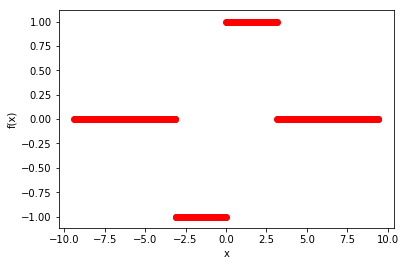
\includegraphics[scale=0.6]{1.png}
		\caption{A plot of $f(x)$ against $x$ }
	\end{figure}
	\item[(b)] Since the funtion is periodic, we can express it in terms of  fourier series.
	\begin{align}
	f(x)=\frac{a_{0}}{2}+ \sum^{\infty}_{n=1}(a_{n} \cos(nx)+ b_{n}\sin(nx)) \label{11}
	\end{align}
		Where:
		\begin{align*}
		a_{n}(x)&=\frac{1}{\pi}\int^{\pi}\limits_{-\pi}f(x)\cos(nx)dx\\
		b_{n}(x)&=\frac{1}{\pi}\int^{\pi}\limits_{-\pi}f(x)\sin(nx)dx\\
		a_{0}&=\frac{1}{\pi}\int^{\pi}\limits_{-\pi}f(x)dx
		\end{align*}
		We want to show that $a_{n}(x)=0$ and $a_{0}=0$, so that the function f(x) is expressed only in sines.\\
		\begin{align*}
			a_{n}&=\frac{1}{\pi}\int^{\pi}\limits_{-\pi}f(x)\cos(nx)dx\\
			&=\frac{1}{\pi}[\int^{0}\limits_{-\pi}-\cos(nx)dx+\int^{\pi}\limits_{0}\cos(nx)dx ]\\
			&=\frac{1}{\pi}[|\frac{-\sin (nx)}{n}|^{0}_{-\pi}+|\frac{\sin (nx)}{n}|^{\pi}_{0} ]\\
			&=0
		\end{align*}
	In a similar way, we compute $a_{0}$;
	\begin{align*}
	a_{0}&=\frac{1}{\pi}\int^{\pi}\limits_{-\pi}f(x)dx\\
	&=\frac{1}{\pi}[\int^{0}\limits_{-\pi}-1dx + \int^{\pi}\limits_{0}1dx ]\\
	&=\frac{1}{\pi}[|-x|^{0}_{-\pi}+|x|^{\pi}_{0}]\\
	&=0
	\end{align*}
	Since $a_{0}$ and $a_{n}$ have been proven to be zero, equation(\ref{11}) now becomes;\\
	\begin{align*}
	f(x)=\sum^{\infty}_{n=1} b_{n}\sin(nx)
	\end{align*}
	\item[(c)]
	The fourier series for f(x) is given by;\\
	\begin{align*}
	b_{n}(x)&=\frac{1}{\pi}\int^{\pi}\limits_{-\pi}f(x)\sin(nx)dx\\
	&=\frac{1}{\pi}[\int^{0}\limits_{-\pi}f(x)\sin(nx)dx + \int^{\pi}\limits_{0}\sin(nx)dx ]\\
	&=\frac{1}{\pi}[\int^{0}\limits_{-\pi}-\sin(nx)dx+\int^{\pi}\limits_{0}\sin(nx)dx ]\\
	&=\frac{1}{\pi}[|\frac{\cos (nx)}{n}|^{0}_{-\pi}+|\frac{-\cos (nx)}{n}|^{\pi}_{0} ]\\
	&=\frac{1}{n\pi}(\cos(0)-\cos(-n\pi))-\frac{1}{n\pi}(\cos(-n\pi)-\cos(0))
	\end{align*}
$\cos(n\pi)=(-1)^{n}$,  $\cos(-n\pi)=(-1)^{n}$, and $\cos(0)=1$.
\begin{align*}
b_{n}&=\frac{1}{n\pi}(1-(-1)^{n}-(-1)^{n}+1)\\
&=\frac{1}{n\pi}(2-2(-1)^{n})\\
&=\frac{2}{n\pi}(1-(-1)^{n}).
\end{align*}
The fourier series of f(x) can be expressed as;
\begin{align*}
f(x)&=\sum^{\infty}_{n=1} b_{n}\sin(nx)\\
&=\sum^{\infty}_{n=1} \frac{2}{n\pi}(1-(-1)^{n}) \sin(nx)
\end{align*}
\end{itemize}
\end{document}